%検証

本章では,SAS-L2を利用したセキュアな組込みシステムをシステム設計を基に実装し,検証を行う.
使用端末,使用センサ,開発環境,テスト結果について述べる.
\section{使用端末}
本研究では,エッジデバイスとしてArduino Leonardoを利用し,3台使用している.
Arduino Leonardoとは,Microchip Technology社のATmega32U4を基に作られたマイクロコントローラーボードである.

\section{使用センサ}
本研究で使用したセンサについて,以下の表\ref{tab:sensor}にまとめる.
\begin{table}[H]
\centering
\caption{使用センサ}
\label{tab:sensor}
\begin{tabular}{|c|c|} \hline
 UV指数センサ & SI1145\\ \hline
 温度センサ & MCP9808\\ \hline
 湿度センサ & HIH-6130\\ \hline
\end{tabular}
\end{table}

\section{開発環境}
本研究の開発環境について,以下の表\ref{tab:kankyo}にまとめる.
\begin{table}[H]
\centering
\caption{開発環境}
\label{tab:kankyo}
\begin{tabular}{|c|c|} \hline
 OS & windows10\\ \hline
 開発環境 & Arduino IDE \\ \hline
 使用言語 & C/C++ \\ \hline
 通信モジュール & ESP-WROOM-02 \\ \hline
\end{tabular}
\end{table}

\section{テスト}
単体テスト,結合テスト,総合テストの順番でテストを行い,テスト結果について
表と図を用いてまとめた.
結合テストと総合テストでは,Arduinoが認証要請を行う際の指定時刻を毎分0秒としてテストを行った.

\subsection{単体テスト}
単体テストでは詳細設計を参考してテストを行った.単体テスト項目と結果を表\ref{tab:tantai_test1},表\ref{tab:tantai_test2}に示す.
通信モジュールであるESP-WROOM-02は,以降でESP8266と定義する.

\begin{table}[H]
\centering
\caption{単体テスト前半}
\label{tab:tantai_test1}
\scalebox{0.8}{
\begin{tabular}{|c|l|c|c|c|c|} \hline
 機能枠&確認内容&結果&確認日&確認者&備考欄\\ \hline\hline
 \multirow{2}{*}{
 \shortstack{
 通信モジュー\\
 ルとの接続}} & 
  \shortstack[l]{
   ArduinoとESP8266を接続した時,ESP8266\\
   との接続が確認できたら,シリアルモニタに\\
   "ESP8266OK"と表示される.} &
   $\bigcirc$ & 2022/1/10 & 浅野& \\ \cline{2-6}
& \shortstack[l]{
   ArduinoとESP8266を接続しなければ,\\
   ESP8266との接続が確認できず,\\
   赤LEDが点滅する.} &
   $\bigcirc$ & 2022/1/10 & 浅野& \\ \hline
 Wi-Fi接続 &
   \shortstack[l]{
   Wi-Fiとの接続ができれば,シリアルモニ\\
   タに"connect success"と\\
   表示される.} &
   $\bigcirc$ & 2022/1/10 & 浅野& \\ \hline
 UDP接続 &
   \shortstack[l]{
   IPアドレス"ntp.nict.jp",ポート番号"123"\\
   へUDP接続が成功すれば,時刻同期処理が\\
   開始される.} &
   $\bigcirc$ & 2022/1/10 & 浅野& \\ \hline
 TCP接続 &
   \shortstack[l]{
   IPアドレス"192.168.2.110",ポート番号\\
   "49152"へTCP接続が成功すれば,シリア\\
   ルモニタに"create tcp ok"と表示\\
   される.} &
   $\bigcirc$ & 2022/1/10 & 浅野& \\ \hline
 \multirow{3}{*}{センサ} &
   Arduinoとセンサが接続している. &
   $\bigcirc$ & 2022/1/10 & 浅野& \\ \cline{2-6}
 & \shortstack[l]{
   Arduinoとセンサが接続されていなけれ\\
   ば,赤LEDが点滅する.} &
   $\bigcirc$ & 2022/1/10 & 浅野&\\ \cline{2-6}
 & センサ値を取得する. &
   $\bigcirc$ & 2022/1/10 & 浅野&\\ \hline
 時刻取得 &
   \shortstack[l]{
   センサ値を取得した時点の年,月,日,時,\\
   分,秒を取得する.} &
   $\bigcirc$ & 2022/1/10 & 浅野& \\ \hline
 \multirow{2}{*}{
 \shortstack[l]{
 認証の際の\\
 $\beta$の演算}}
 & \shortstack[l]{
  $A_{n+1} \leftarrow \alpha \oplus A_n \oplus M_n$ の演算\\
   結果が正しい.演算結果は128bitである. }
 & $\bigcirc$ & 2022/1/10 & 浅野& 
   \shortstack[l]{
   図\ref{fig:alpha}\\
   図\ref{fig:beta_An}\\
   図\ref{fig:beta_Mn}\\
   図\ref{fig:beta_Am}} \\ \cline{2-6}
 & \shortstack[l]{
   $\beta \leftarrow A_{n+1} +A_n$の\\
   演算結果が正しい.演算結果は128bit\\
   である.} &
   $\bigcirc$ & 2022/1/10 & 浅野 & 
   \shortstack[l]{
   図\ref{fig:beta_An}\\
   図\ref{fig:beta_Am}\\
   図\ref{fig:beta}}\\ \hline
 \shortstack[l]{ 
 認証の際の\\
 次回秘匿情報\\
 の計算} &
   \shortstack[l]{
   $M_{n+1} \leftarrow A_n + M_n$の演算が正しい.\\
   演算結果は128bitである.} &
   $\bigcirc$ & 2022/1/10 & 浅野&
   \shortstack[l]{
   図\ref{fig:beta_An}\\
   図\ref{fig:beta_Mn}\\
   図\ref{fig:ninsyo_Mm}}\\ \hline 
\shortstack[l]{
 認証成功時の\\
 認証情報$A_n$,$A_{n+1}$,\\
 秘匿情報$M_n$の\\
 更新}
 & \shortstack[l]{
   n回目認証成功時の$A_n$,$A_{n+1}$,$M_{n+1}$を\\
   EEPROMのアドレス0-15,16-31,32-47に\\
   それぞれ書き込む.} &
   $\bigcirc$ & 2022/1/10 & 浅野 &\\ \hline
$SD$の生成 &
   \shortstack[l]{
   float型(32bit)センサ値と,int型(16bit)\\
   の年,int$8_t$型(8bit)の月,日,時,分,秒を\\
   unsigned char型の128bit配列に格納\\
   される.}&
   $\bigcirc$ & 2022/1/10 & 浅野&\\ \hline
\end{tabular}
}
\end{table}

\begin{table}[H]
\centering
\caption{単体テスト後半}
\label{tab:tantai_test2}
\scalebox{0.8}{
\begin{tabular}{|c|l|c|c|c|c|} \hline
 機能枠&確認内容&結果&確認日&確認者&備考欄\\ \hline\hline
 \shortstack[l]{ 
 暗号化通信の際の\\
 $\gamma$の演算}&
   \shortstack[l]{
   $\gamma \leftarrow SD \oplus A_{n+1} \oplus A_n$\\
   の演算結果が正しい.演算結果は128bit\\
   である.} &
   $\bigcirc$ & 2022/1/10 & 浅野&
   \shortstack[l]{
   図\ref{fig:SD}\\
   図\ref{fig:beta_Am}\\
   図\ref{fig:beta_An}\\
   図\ref{fig:gamma}}\\ \hline
 \shortstack[l]{
 暗号化通信の際の\\
 認証情報$A_{n+2}$\\
 の演算} &
   \shortstack[l]{  
   $A_{n+2} \leftarrow \alpha \oplus A_{n+1} \oplus M_{n+1}$\\
   の演算結果が正しい.演算結果は128bi\\
   tである.}&
   $\bigcirc$ & 2022/1/10 & 浅野&
   \shortstack[l]{
   図\ref{fig:ango_alpha}\\
   図\ref{fig:beta_Am}\\
   図\ref{fig:ninsyo_Mm}\\
   図\ref{fig:ango_Al}}\\ \hline
 \shortstack[l]{ 
 暗号化通信の際の\\
 次回秘匿情報\\
 の計算} &
   \shortstack[l]{
   $M_{n+2} \leftarrow A_{n+1} + M_{n+1}$の演算が正しい.\\
   演算結果は128bitである.} &
   $\bigcirc$ & 2022/1/10 & 浅野&
   \shortstack[l]{
   図\ref{fig:beta_Am}\\
   図\ref{fig:ninsyo_Mm}\\
   図\ref{fig:ango_Mm}}\\ \hline
 \shortstack[l]{ 
 暗号化通信の際の\\
 認証情報,\\
 秘匿情報の更新} &
   \shortstack[l]{   
   10回目暗号化終了時の$A_n$,$A_{n+1}$,$M_{n+1}$を\\
   EEPROMのアドレス0-15,16-31,32-47\\
   それぞれ書き込む.} &
   $\bigcirc$ & 2022/1/10 & 浅野&\\ \hline
\end{tabular}
}
\end{table}

認証の際にArduinoが生成する$\beta$の演算は,$A_{n+1} \leftarrow \alpha \oplus A_n \oplus M_n$,$\beta \leftarrow A_{n+1} + A_n$と書ける.$A_{n+1} \leftarrow \alpha \oplus A_n \oplus M_n$の演算は,シリアルモニタに表示させたビット列である図\ref{fig:alpha}と図\ref{fig:beta_An},図\ref{fig:beta_Mn}の3つの排他的論理和を演算し,その演算結果が図\ref{fig:beta_Am}になったことから,正しく演算されたと分かる.
$\beta \leftarrow A_{n+1} + A_n$の演算は,シリアルモニタに表示させたビット列である図\ref{fig:beta_Am}と図\ref{fig:beta_An}の算術加算の結果が図\ref{fig:beta}になったことから,正しく演算されたと分かる.\\
認証の際に行う次回秘匿情報の演算は$M_{n+1} \leftarrow A_n + M_n$であり,シリアルモニタに表示させたビット列である図\ref{fig:beta_An}と図\ref{fig:beta_Mn}の算術加算の結果が図\ref{fig:ninsyo_Mm}になったことから,正しく演算されたと分かる.\\
\begin{figure}[H]
\begin{minipage}{0.33\hsize}
\centering
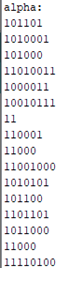
\includegraphics{alpha.png}
\caption{認証の際の$\alpha$}
\label{fig:alpha}
\end{minipage}
\begin{minipage}{0.33\hsize}
\centering
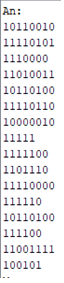
\includegraphics{beta_An.png}
\caption{認証情報$A_n$}
\label{fig:beta_An}
\end{minipage}
\begin{minipage}{0.33\hsize}
\centering
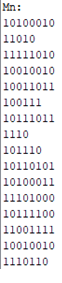
\includegraphics{beta_Mn.png}
\caption{秘匿情報$M_n$}
\label{fig:beta_Mn}
\end{minipage}
\end{figure}

\begin{figure}[H]
\begin{minipage}{0.33\hsize}
\centering
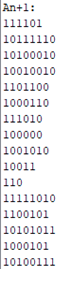
\includegraphics{beta_Am.png}
\caption{認証情報$A_{n+1}$}
\label{fig:beta_Am}
\end{minipage}
\begin{minipage}{0.33\hsize}
\centering
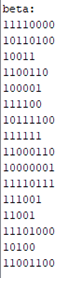
\includegraphics{beta.png}
\caption{$\beta$}
\label{fig:beta}
\end{minipage}
\begin{minipage}{0.33\hsize}
\centering
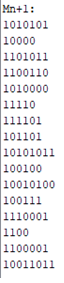
\includegraphics{ninsyo_Mm.png}
\caption{秘匿情報$M_{n+1}$}
\label{fig:ninsyo_Mm}
\end{minipage}
\end{figure}


暗号化の際に生成する$\gamma$の演算は$\gamma \leftarrow SD \oplus A_{n+1} \oplus A_n$である.
$\gamma \leftarrow SD \oplus A_{n+1} \oplus A_n$の演算は,シリアルモニタに表示させたビット列である図\ref{fig:SD}と図\ref{fig:beta_Am},図\ref{fig:beta_An}の3つの排他的論理和を演算し,その演算結果が図\ref{fig:gamma}になったことから,正しく演算されたと分かる.\\
暗号化の際に生成する認証情報の演算は$A_{n+2} \leftarrow \alpha \oplus A_{n+1} \oplus M_{n+1}$であり,$A_{n+2} \leftarrow \alpha \oplus A_{n+1} \oplus M_{n+1}$の演算は,シリアルモニタに表示させたビット列である図\ref{fig:ango_alpha}と図\ref{fig:beta_Am},図\ref{fig:ninsyo_Mm}の3つの排他的論理和の結果が図\ref{fig:ango_Al}になったことから,正しく演算されたと分かる.\\
暗号化の際に生成する次回秘匿情報の演算は$M_{n+2} \leftarrow A_{n+1} + M_{n+1}$であり,シリアルモニタに表示させたビット列である図\ref{fig:beta_Am}と図\ref{fig:ninsyo_Mm}の算術加算の結果が図\ref{fig:ango_Mm}になったことから,正しく演算されたと分かる.図\ref{fig:ango_Mm}では,$M_{n+1} \leftarrow M_{n+2}$で秘匿情報$M_{n+1}$に更新しているため,演算結果は$M_{n+1}$としてモニタに表示されている.\\

\begin{figure}[H]
\begin{minipage}{0.5\hsize}
\centering
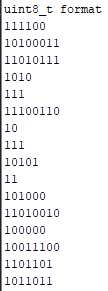
\includegraphics{SD.png}
\caption{$SD$}
\label{fig:SD}
\end{minipage}
\begin{minipage}{0.5\hsize}
\centering
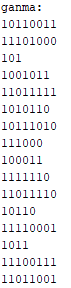
\includegraphics{gamma.png}
\caption{$\gamma$}
\label{fig:gamma}
\end{minipage}
\end{figure}

\begin{figure}[H]
\begin{minipage}{0.33\hsize}
\centering
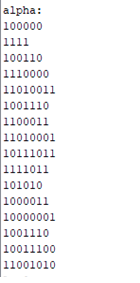
\includegraphics{ango_alpha.png}
\caption{暗号化通信の際の$\alpha$}
\label{fig:ango_alpha}
\end{minipage}
\begin{minipage}{0.33\hsize}
\centering
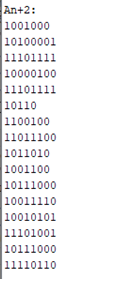
\includegraphics{ango_Al.png}
\caption{認証情報$A_{n+2}$}
\label{fig:ango_Al}
\end{minipage}
\begin{minipage}{0.33\hsize}
\centering
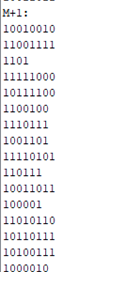
\includegraphics{ango_Mm.png}
\caption{秘匿情報$M_{n+2}$}
\label{fig:ango_Mm}
\end{minipage}
\end{figure}

\subsection{結合テスト}
結合テストでは基本設計を参考してテストを行った.結合テスト項目と結果を表\ref{tab:ketugo_test}に示す.
Arduinoはユーザー,Raspberry Piはサーバーと定義する.
\begin{table}[H]
\centering
\caption{結合テスト}
\label{tab:ketugo_test}
\scalebox{0.8}{
\begin{tabular}{|c|l|c|c|c|c|} \hline
 機能枠&確認内容&結果&確認日&確認者&備考欄\\ \hline\hline
 \multirow{5}{*}{認証} &
   認証要請の送受信を行う. &
   $\bigcirc$ & 2022/1/14 &
   \shortstack[l]{
   浅野\\
   内山田}&\\ \cline{2-6}
 & \shortstack[l]{
   認証の際,$\alpha$の送受信を行い,サーバーが送信\\
   したデータと,ユーザーが受信したデータ\\
   が一致している.} &
   $\bigcirc$ & 2022/1/14 &
   \shortstack[l]{
   浅野\\
   内山田}&
   \shortstack[l]{
   図\ref{fig:ninsyo_server_alpha}\\
   図\ref{fig:ninsyo_uv_alpha}}\\ \cline{2-6}
 & \shortstack[l]{
   認証の際,$\beta$の送受信を行い,ユーザーが送信\\
   したデータと,サーバーが受信したデータ\\
   が一致している.} &
   $\bigcirc$ & 2022/1/14 &
   \shortstack[l]{
   浅野\\
   内山田} &
   \shortstack[l]{
   図\ref{fig:ninsyo_uv_beta}\\
   図\ref{fig:ninsyo_server_beta}}\\ \cline{2-6}
 & 認証結果の送受信を行う. &
   $\bigcirc$ & 2022/1/14 &
   \shortstack[l]{
   浅野\\
   内山田}&\\ \cline{2-6}
 & \shortstack[l]{
   ユーザーで演算した\\
   認証情報$A_{n+1}$,秘匿情報$M_{n+1}$と,\\
   サーバーで演算した\\
   認証情報$A_{n+1}$,秘匿情報$M_{n+1}$が\\
   一致している.} &
   $\bigcirc$ & 2022/1/14 &
   \shortstack[l]{
   浅野\\
   内山田}&\\ \hline
\multirow{4}{*}{暗号化通信} & 
 \shortstack[l]{
   $\gamma$の送受信を行い,ユーザーが送信したデー\\
   タと,サーバーが受信したデータが一致し\\
   ている.} &
   $\bigcirc$ & 2022/1/14 &
   \shortstack[l]{
   浅野\\
   内山田}&
 \shortstack[l]{
   図\ref{fig:ninsyo_uv_gamma}\\
   図\ref{fig:ninsyo_server_gamma}}\\ \cline{2-6}
 & \shortstack[l]{
   ユーザーが取得したセンシングデータと日\\
   時が,データベースに保存されたセンシング\\
   データと日時と一致している. } &
   $\bigcirc$ & 2022/1/14 &
   \shortstack[l]{
   浅野\\
   内山田}&
 \shortstack[l]{
   図\ref{fig:ango_uv_sd}\\
   図\ref{fig:ango_server_sd}}\\ \cline{2-6}
 & \shortstack[l]{
   暗号化通信の際,$\alpha$の送受信を行い,サーバ\\
   ーが送信したデータと,ユーザーが受信した\\
   データが一致している.} &
   $\bigcirc$ & 2022/1/14 &
   \shortstack[l]{
   浅野\\
   内山田}&
   \shortstack[l]{
   図\ref{fig:ango_server_alpha}\\
   図\ref{fig:ango_uv_alpha}}\\ \cline{2-6}
 & \shortstack[l]{
   暗号化通信終了後,ユーザーとサーバーがそ\\
   れぞれ演算を行った認証情報$A_n$と秘匿情報\\
   $M_n$が一致している.} &
   $\bigcirc$ & 2022/1/14 &
   \shortstack[l]{
   浅野\\
   内山田}&\\ \hline
 \end{tabular}
}
\end{table}



サーバーが送信した$\alpha$は図\ref{fig:ninsyo_server_alpha}であり,
ユーザーが受信した$\alpha$は図\ref{fig:ninsyo_uv_alpha}であることから,
$\alpha$の値が一致しており,送受信が正しく行われたことが分かる.
\begin{figure}[H]
\begin{center}
	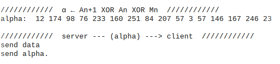
\includegraphics[width=10cm]{ninsyo_server_alpha.png}
	\caption{認証の際にサーバーが送信した$\alpha$}
	\label{fig:ninsyo_server_alpha}
\end{center}
\end{figure}
\begin{figure}[H]
\begin{center}
	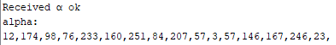
\includegraphics[width=10cm]{ninsyo_uv_alpha.png}
	\caption{認証の際にユーザーが受信した$\alpha$}
	\label{fig:ninsyo_uv_alpha}
\end{center}
\end{figure}

ユーザーが送信した$\beta$は図\ref{fig:ninsyo_uv_beta}であり,
ユーザーが受信した$\beta$は図\ref{fig:ninsyo_server_beta}であることから,
$\beta$の値が一致しており,送受信が正しく行われたことが分かる.

\begin{figure}[H]
\begin{center}
	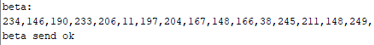
\includegraphics[width=10cm]{ninsyo_uv_beta.png}
	\caption{認証の際にユーザーが送信した$\beta$}
	\label{fig:ninsyo_uv_beta}
\end{center}
\end{figure}
\begin{figure}[H]
\begin{center}
	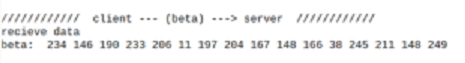
\includegraphics[width=10cm]{ninsyo_server_beta.png}
	\caption{認証の際にサーバーが受信した$\beta$}
	\label{fig:ninsyo_server_beta}
\end{center}
\end{figure}


ユーザーが送信した$\gamma$は図\ref{fig:ninsyo_uv_gamma}であり,
ユーザーが受信した$\gamma$は図\ref{fig:ninsyo_server_gamma}であることから,
$\gamma$の値が一致しており,送受信が正しく行われたことが分かる.

\begin{figure}[H]
\begin{center}
	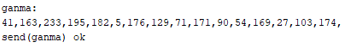
\includegraphics[width=10cm]{ninsyo_uv_gamma.png}
	\caption{暗号化通信の際にユーザーが送信した$\gamma$}
	\label{fig:ninsyo_uv_gamma}
\end{center}
\end{figure}
\begin{figure}[H]
\begin{center}
	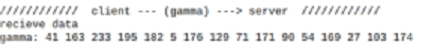
\includegraphics[width=10cm]{ninsyo_server_gamma.png}
	\caption{暗号化通信の際にサーバーが受信した$\gamma$}
	\label{fig:ninsyo_server_gamma}
\end{center}
\end{figure}

ある時点でユーザーが取得したセンシングデータと日時は図\ref{fig:ango_uv_sd}であり,
サーバーがデータベースに保存したセンシングデータと日時は図\ref{fig:ango_server_sd}
のデータベースに含まれていることから,センシングデータと日時が正しくデータベースに保存されたことが分かる.

\begin{figure}[H]
\begin{center}
	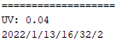
\includegraphics[width=4cm]{ango_uv_sd.png}
	\caption{ユーザーが取得したセンシングデータと日時}
	\label{fig:ango_uv_sd}
\end{center}
\end{figure}
\begin{figure}[H]
\begin{center}
	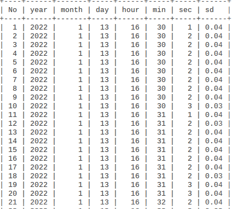
\includegraphics[width=10cm]{ango_server_sd.png}
	\caption{データベースに保存されたセンシングデータと日時}
	\label{fig:ango_server_sd}
\end{center}
\end{figure}

暗号化通信の際にサーバーが送信した$\alpha$は図\ref{fig:ango_server_alpha}であり,
ユーザーが受信した$\alpha$は図\ref{fig:ango_uv_alpha}であることから,
$\alpha$の値が一致しており,送受信が正しく行われたことが分かる.

\begin{figure}[H]
\begin{center}
	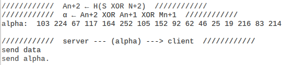
\includegraphics[width=10cm]{ango_server_alpha.png}
	\caption{暗号化通信の際にサーバーが送信した$\alpha$}
	\label{fig:ango_server_alpha}
\end{center}
\end{figure}
\begin{figure}[H]
\begin{center}
	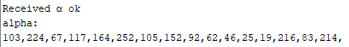
\includegraphics[width=10cm]{ango_uv_alpha.png}
	\caption{暗号化通信の際にユーザーが受信した$\alpha$}
	\label{fig:ango_uv_alpha}
\end{center}
\end{figure}

\subsection{総合テスト}
総合テストでは要件定義を参考してテストを行った.総合テスト項目と結果を表\ref{tab:sogo_test}に示す.
Arduinoはユーザー,Raspberry Piはサーバーと定義する.

\begin{table}[htbp]
\centering
\caption{総合テスト}
\label{tab:sogo_test}
\scalebox{0.7}{
\begin{tabular}{|c|l|c|c|c|c|} \hline
 機能枠&確認内容&結果&確認日&確認者&備考欄\\ \hline\hline
  \multirow{12}{*}{認証}
& ユーザーは起動後,1度時刻同期を行う.  &
   $\bigcirc$ & 2022/1/14 &
   \shortstack[l]{
   浅野\\
   内山田}&\\ \cline{2-6}
 & ユーザーが指定した時間に認証要請を送信する. &
   $\bigcirc$ & 2022/1/14 &
   \shortstack[l]{
   浅野\\
   内山田}&\\ \cline{2-6}
 & \shortstack[l]{
   複数のユーザーは同時刻に認証要請を送信するので,\\
   一台の認証が終了するまで,その他のユーザーは待機状態になる.} &
   $\bigcirc$ & 2022/1/14 &
   \shortstack[l]{
   浅野\\
   内山田}&\\ \cline{2-6}
 & ユーザーが認証処理を行っている. &
   $\bigcirc$ & 2022/1/14 &
   \shortstack[l]{
   浅野\\
   内山田}
& 図\ref{fig:sogo_ninsyo_uv}\\ \cline{2-6}
 & ユーザーが認証結果をモニタに表示している. &
   $\bigcirc$ & 2022/1/14 &
   \shortstack[l]{
   浅野\\
   内山田}&\\ \cline{2-6}
 & \shortstack[l]{ 
   認証が成功した場合,ユーザーがSAS-L2に基づいた\\
   暗号化通信を行う.} &
   $\bigcirc$ & 2022/1/14 &
   \shortstack[l]{
   浅野\\
   内山田}
 & \\ \cline{2-6}
 & \shortstack[l]{
   認証が失敗した場合,ユーザーはコネクションを切断して\\
  認証要請送信から再度開始する.} &
   $\bigcirc$ & 2022/1/14 &
   \shortstack[l]{
   浅野\\
   内山田}&\\ \cline{2-6}
 & サーバーが起動したら,受信待ち状態になる. &
   $\bigcirc$ & 2022/1/14 &
   \shortstack[l]{
   浅野\\
   内山田}&\\ \cline{2-6}
 & サーバーが認証要請受信後,認証処理を行っている. &
   $\bigcirc$ & 2022/1/14 &
   \shortstack[l]{
   浅野\\
   内山田}&
図\ref{fig:sogo_ninsyo_server_1}\\ \cline{2-6}
 & サーバーが認証結果をモニタに表示している. &
   $\bigcirc$ & 2022/1/14 &
   \shortstack[l]{
   浅野\\
   内山田}&\\ \cline{2-6} 
& \shortstack[l]{ 
   認証が成功した場合,サーバーがSAS-L2に基づいた暗号化通信を\\
   行う.} &
   $\bigcirc$ & 2022/1/14 &
   \shortstack[l]{
   浅野\\
   内山田}&\\ \cline{2-6}
 & \shortstack[l]{
   認証が失敗した場合,サーバーはコネクションを切断して\\
   認証要請の待ち状態となる.} &
   $\bigcirc$ & 2022/1/14 &
   \shortstack[l]{
   浅野\\
   内山田}&\\ \hline
 \multirow{9}{*}{暗号化通信}
 & ユーザーはセンシングデータを取得する. &
   $\bigcirc$ & 2022/1/14 &
   \shortstack[l]{
   浅野\\
   内山田}&\\ \cline{2-6}
 & \shortstack[l]{
   ユーザーは,シリアルモニタに取得したセンシングデータと\\
   センシングデータ取得日時を表示する.} &
   $\bigcirc$ & 2022/1/14 &
   \shortstack[l]{
   浅野\\
   内山田}
& \shortstack[l]{
図\ref{fig:pc_uv}\\
図\ref{fig:pc_mcp}\\
図\ref{fig:pc_hih}}\\ \cline{2-6}
 & \shortstack[l]{
   ユーザーはセンシングデータと日時を暗号化して\\
   サーバーへ送信する.} &
   $\bigcirc$ & 2022/1/14 &
   \shortstack[l]{
   浅野\\
   内山田}&\\ \cline{2-6}
 & ユーザーは暗号化通信を10回行う. &
   $\bigcirc$ & 2022/1/14 &
   \shortstack[l]{
   浅野\\
   内山田}&\\ \cline{2-6}
 & ユーザーは暗号化通信後,コネクションを切断する. &
   $\bigcirc$ & 2022/1/14 &
   \shortstack[l]{
   浅野\\
   内山田}&\\ \cline{2-6}
 & サーバーはセンシングデータと日時を復号する. &
   $\bigcirc$ & 2022/1/14 &
   \shortstack[l]{
   浅野\\
   内山田}&\\ \cline{2-6}
 & \shortstack[l]{
   サーバーはセンシングデータと取得日時を保存する際に,\\
   ユーザーごとのテーブルに分けて保存する.}  &
   $\bigcirc$ & 2022/1/14 &
   \shortstack[l]{
   浅野\\
   内山田}
 & \shortstack[l]{
図\ref{fig:db_uv}\\
図\ref{fig:db_hih}\\
図\ref{fig:db_mcp}}\\ \cline{2-6}
 & サーバーは暗号化通信を10回行う. &
   $\bigcirc$ & 2022/1/14 &
   \shortstack[l]{
   浅野\\
   内山田}&\\ \cline{2-6}
 &  \shortstack[l]{
   サーバーは暗号化通信後,コネクションを切断し\\
   認証要請待ち状態となる.} &
   $\bigcirc$ & 2022/1/14 &
   \shortstack[l]{
   浅野\\
   内山田}&\\ \hline
 \multirow{3}{*}{通信}
 & \shortstack[l]{
   ユーザーで,何らかのエラーが発生した場合,\\
   赤LEDを点滅させる.} &
   $\bigcirc$ & 2022/1/14 &
   \shortstack[l]{
   浅野\\
   内山田}&\\ \cline{2-6}
 & \shortstack[l]{
   サーバーは,5秒以上データを受信できなけ\\
   れば,コネクションを切断して認証要請\\
   受信の待機状態となる.} &
   $\bigcirc$ & 2022/1/14 &
   \shortstack[l]{
   浅野\\
   内山田}&\\ \cline{2-6}
& \shortstack[l]{
   3台のユーザーが同時刻に認証要請を送信した場合,\\
   3台のユーザーとの通信が10秒以内に完了する.}&
   $\bigcirc$ & 2022/1/14 &
   \shortstack[l]{
   浅野\\
   内山田}&\\ \hline
\end{tabular}
}
\end{table}
図\ref{fig:sogo_ninsyo_server_1}はサーバーのID:1のユーザーとの認証処理の結果であり,
図\ref{fig:sogo_ninsyo_uv}はID:1のユーザーの認証処理の結果をモニタに表示した図である.
サーバーは認証要請を受信後,生成した認証情報$A_{n+1}$を基に$\alpha$を生成し,ユーザーに送信している.
そして,サーバーはユーザーから$\beta$を受信し,認証結果をユーザーへ送信していると分かる.
ユーザーは認証要請を送信後,サーバーから受信した$\alpha$を基に$\beta$を生成し,サーバーに送信している.そして,ユーザーはサーバーから認証結果を受信し,認証結果から認証が成功したと分かる.
サーバーとID:2,ID:3の間での認証処理についても,同様に認証が成功したことを確認した.

\begin{figure}[H]
\begin{center}
	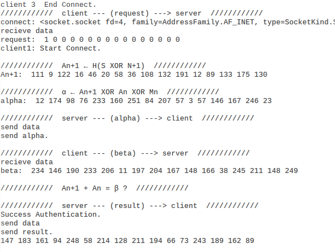
\includegraphics[width=10cm]{sogo_ninsyo_server_1.png}
	\caption{サーバーの認証結果}
	\label{fig:sogo_ninsyo_server_1}
\end{center}
\end{figure}
\begin{figure}[H]
\begin{center}
	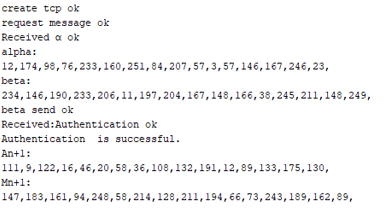
\includegraphics[width=10cm]{sogo_ninsyo_uv.png}
	\caption{ユーザーの認証結果}
	\label{fig:sogo_ninsyo_uv}
\end{center}
\end{figure}


ユーザーが取得したセンシングデータと日時は図\ref{fig:pc_uv}と図\ref{fig:pc_mcp},図\ref{fig:pc_hih}のようにシリアルモニタに表示されることが確認された.示した図はそれぞれある時点のものである.
サーバーがデータベースに保存したセンシングデータと日時は図\ref{fig:db_uv}と図\ref{fig:db_hih},
図\ref{fig:db_mcp}のようにユーザーのIDごとにテーブルに分て保存されていることが分かる.
また,ユーザーが取得したセンシングデータがデータベースに保存されていることから,ユーザーが取得したセンシングデータを暗号化してサーバーに送信し,サーバーがセンシングデータを復号できたことが分かる.

\begin{figure}[H]
\begin{center}
	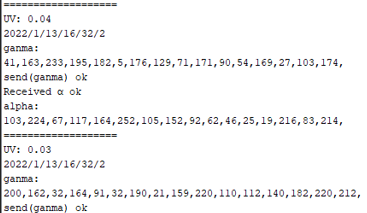
\includegraphics[width=10cm]{pc_uv.png}
	\caption{ID:1のシリアルモニタ}
	\label{fig:pc_uv}
\end{center}
\end{figure}
\begin{figure}[H]
\begin{center}
	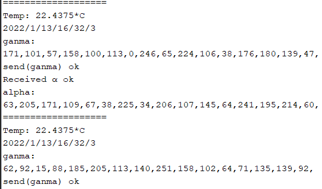
\includegraphics[width=10cm]{pc_mcp.png}
	\caption{ID:2のシリアルモニタ}
	\label{fig:pc_mcp}
\end{center}
\end{figure}
\begin{figure}[H]
\begin{center}
	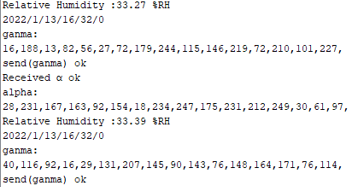
\includegraphics[width=10cm]{pc_hih.png}
	\caption{ID:3のシリアルモニタ}
	\label{fig:pc_hih}
\end{center}
\end{figure}

\begin{figure}[H]
\begin{center}
	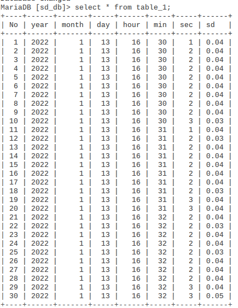
\includegraphics[width=10cm]{db_uv.png}
	\caption{データベースのID:1のテーブル}
	\label{fig:db_uv}
\end{center}
\end{figure}
\begin{figure}[H]
\begin{center}
	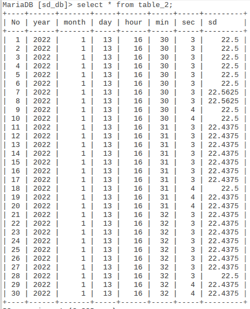
\includegraphics[width=10cm]{db_hih.png}
	\caption{データベースのID:2のテーブル}
	\label{fig:db_hih}
\end{center}
\end{figure}
\begin{figure}[H]
\begin{center}
	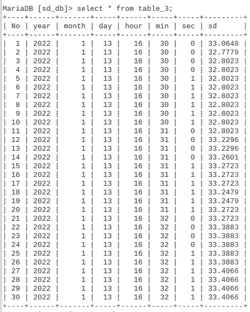
\includegraphics[width=10cm]{db_mcp.png}
	\caption{データベースのID:3のテーブル}
	\label{fig:db_mcp}
\end{center}
\end{figure}

\section{考察}
本節では,IoTにおけるセンシングデバイスでのセキュアなデータ通信の
実装での考察と問題点,今後の課題について述べる.

まず,本研究で開発したシステムの考察を述べる.
本研究では,SAS-L2認証方式をセンシングデバイスに実装することで,
デバイス間の認証とセンシングデータの暗号化通信方法の実現に成功した.
具体的に,認証については図\ref{fig:sogo_ninsyo_server_1}と図\ref{fig:sogo_ninsyo_uv}を用いて示したように,認証が成功したことからSAS-L2認証の実装が実現できたことが分かる.
そして,暗号化通信では,センシングデバイスが取得したセンシングデータを格納した$SD$と認証情報$A_n$と認証情報$A_{n+1}$の排他的論理和をサーバーへ送信し,サーバーがセンシングデータを復号してデータベースへ保存できたことからセンシングデバイスへの暗号化通信方法の実装が実現できたと分かる.

次に,本システムの問題点と今後の課題について述べる.
問題点の1つ目として,本研究ではセンシングデバイスがSAS-L2認証を用いてサーバーとのセキュアなデータ通信
を行うにあたり,初期認証情報と初期秘匿情報がセンシングデバイスに書き込まれていることが前提条件であることである.
実際では,センシングデバイスを生産するにあたり,初期情報が書き込まれているなら前提条件が満たされているが,
初期情報が書き込まれていないセンシングデバイスに関しては,安全な方法で初期情報を取得しなければならない.
安全な方法により初期情報を取得しなければ,悪意のある第三者により初期情報が盗聴され,
以後の認証・暗号化通信も盗聴・改ざんされる可能性がある.
初期情報が書き込まれていないセンシングデバイスである場合は,
初期情報を取得する安全な方法を確保しなければならないことが今後の課題である.


本研究ではエッジデバイスとしてArduino Leonardoを使用したが,Arduinoは電源を切った場合に初期化するため,
認証を行う度に認証情報と秘匿情報を不揮発性メモリに書き込まなければならない.
問題点の2つ目として,このようにセンシングデバイスが電源を切るたびに初期化してしまうものであった場合,
不揮発性メモリを使用しなくてはならないことである.不揮発性メモリは,デバイスの電源が切れても初期化されない
が,書き込み回数には限界がある.デバイスにより不揮発性メモリの寿命も様々であるが,認証回数が増える程に
メモリへの書き込み回数も増えるため,メモリの寿命が短くなる.
不揮発性メモリへの書き込みができなくなれば,認証・暗号化通信もできなくなるため,
一定時間内の認証の回数を決定する際,不揮発性メモリの書き込み回数の限界を考慮しなければならないことが課題である.

